%%%%%%%%%%%%%%%%%%%%%%%%%%%%%%%%%%%%%%%%%%%%%%%%%%%%%%%%%%%%%%%%%%%%%%%%%%%%%%%%
%2345678901234567890123456789012345678901234567890123456789012345678901234567890
%        1         2         3         4         5         6         7         8

%\documentclass[letterpaper, 10 pt, conference]{ieeeconf}  % Comment this line out if you need a4paper
\documentclass[a4paper, 10pt, conference]{ieeeconf}      % Use this line for a4 paper
\IEEEoverridecommandlockouts                              % This command is only needed if 
                                                          % you want to use the \thanks command
\overrideIEEEmargins                                      % Needed to meet printer requirements.
\usepackage{lipsum,graphicx}
\usepackage{here}
\usepackage{subcaption}
\usepackage{url}
\usepackage{comment}
\usepackage[maxfloats=256]{morefloats}
\usepackage{multirow}
\usepackage[table,xcdraw]{xcolor}
\usepackage{stfloats}

\IEEEoverridecommandlockouts                              % This command is only needed if 
                                                          % you want to use the \thanks command
\overrideIEEEmargins                                      % Needed to meet printer requirements.




\title{\LARGE \bf
DNN Based Camera Attitude Estimation \\ Using Aggregated Information from Camera and Depth Images
}


\author{Hibiki Kawai$^{1}$ and Yoji Kuroda$^{2}$% <-this % stops a space
\thanks{$^{1}$Department of Mechanical Engineering, Graduate School of Science and Engineering, Meiji University. Higashi-Mita1-1-1, Tama Ward, Kawasaki City, Kanagawa Prefecture, Japan.
}
\thanks{$^{2}$Department of Mechanical Engineering, School of Science and Technology, Meiji University. Higashi-Mita1-1-1, Tama Ward, Kawasaki City, Kanagawa Prefecture, Japan.
}
\thanks{*Contact to corresponding author:
        {\tt\small ce212026@meiji.ac.jp}}}%}% <-this stops a space



\begin{document}



\maketitle
\thispagestyle{empty}
\pagestyle{empty}


%%%%%%%%%%%%%%%%%%%%%%%%%%%%%%%%%%%%%%%%%%%%%%%%%%%%%%%%%%%%%%%%%%%%%%%%%%%%%%%%
\begin{abstract}

In this paper, we propose a camera attitude estimation network that features aggregated information extracted from camera and depth images. When robots estimate attitude, the estimation method using IMU or gyro-sensors like robots widely used is affected by noise generated from the ground, which makes the attitude estimation difficult. Although there are several methods for estimating the attitude of ground robots, a camera image-based estimation method using deep learning has been studied in recent years. Previous studies have improved the accuracy of the attitude estimation in a known environment, but that in an unknown environment remains low. When making an attitude estimation in an unknown environment, it is important to have an assumption of the terrain, such as that walls are approximately vertical to the ground. Our research uses as input two types of images: a camera image for landscape information and a depth image for terrain information. We propose a network that incorporates a feature extractor that uses cross-reference information of different modalities obtained from these two types of images and a classification type output layer. This network aims to improve the accuracy of attitude estimation in unknown environments. Source code of proposed method is available at \url{https://github.com/Hibiki1020/camera_and_depth_image_attitude_estimator}

\end{abstract}

%本論文ではOCRのアイデアをベースとしたクラス分類ニューラルネットワークによるカメラ姿勢推定手法を提案する。
%ロボットattitudeを推定する場合、ドローンのようにIMUやジャイロセンサを用いたattitude推定手法では、地面から発生するノイズに影響されてattitude推定が困難なものになる。
%地上ロボットのattitude estimation手法は複数存在するが、深層学習を使用したcamera imageによる推定手法の研究が近年研究されている。これまでの研究によってknown environmentにおけるattitude推定の精度は改善したが, unknown environmentにおけるattitude estimationの精度は依然低いままであった。
%unknown environmentでのattitude estimationを行うときに重要となるのは, 壁は地面に対して垂直であるなどの地形についての前提知識である。
%本研究は、風景情報を得られるcamera imageと地形情報を得られるdepth imageの二つを入力として利用する。この二種類の画像から得られるmodalityの異なる情報を相互に参照しあうfeature extractorとclassification type output layerを取り入れたネットワークを提案する。このネットワークによってunknown environmentにおけるattitude estimationの精度改善を狙う

%%%%%%%%%%%%%%%%%%%%%%%%%%%%%%%%%%%%%%%%%%%%%%%%%%%%%%%%%%%%%%%%%%%%%%%%%%%%%%%%
\section{Introduction}

Attitude estimation is an essential task in robotics. There is a ground robot that capable of high maneuverability by freely tilting its upper body as shown in Fig.\ref{fig:CCV}. In such robots, a failure of the attitude estimation has serious consequences, such as falls. Usually, robots use sensors such as IMU to estimate their attitude. However, in the case of ground robots, drift and bias due to unevenness and slippage of the ground can make attitude estimation difficult\cite{Vaganay1993MobileRA}. This means that the estimation of the attitude by relying on the internal sensor is difficult.

   \begin{figure}[thpb]
      \centering
      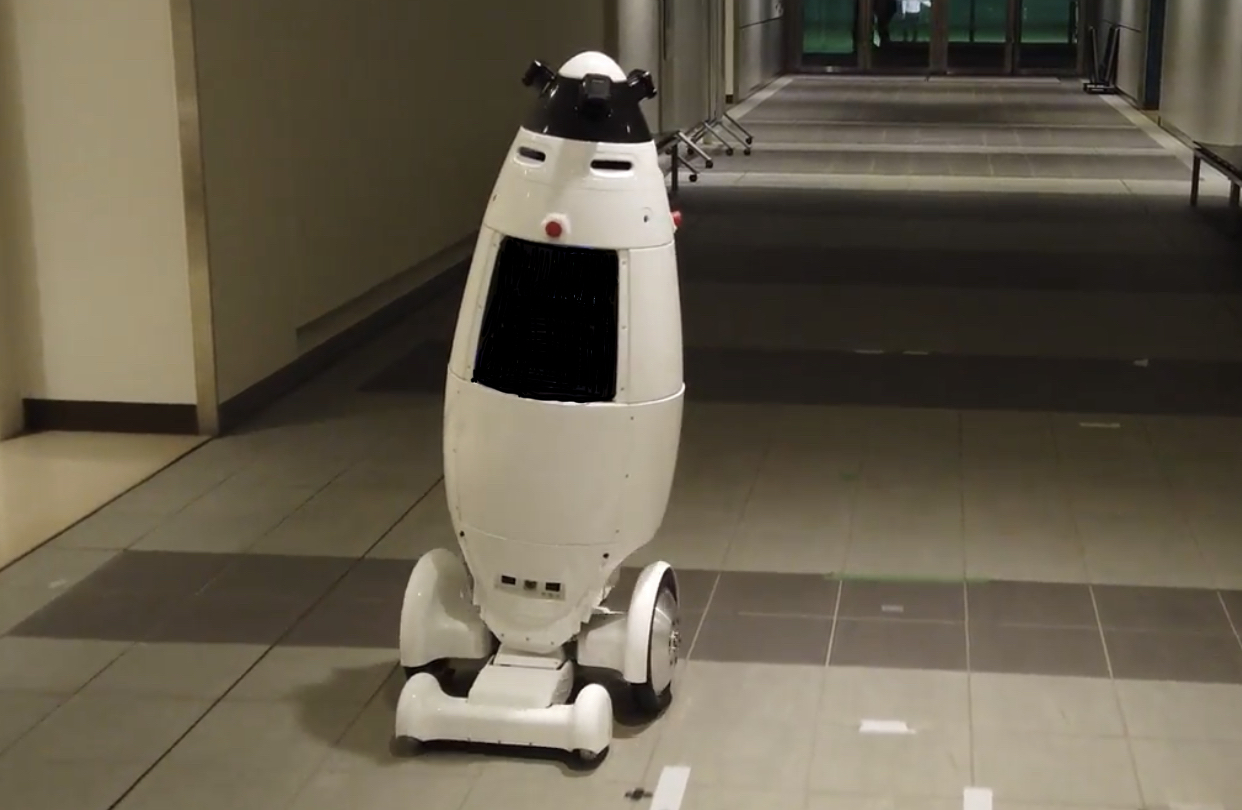
\includegraphics[scale=0.13]{./figure/1_introduction/CCV.jpg}
      \caption{Robots can perform high maneuverability by freely
tilting their upper body}
      \label{fig:CCV}
   \end{figure}

To address this problem, there are much research on attitude estimation using SLAM techniques\cite{thrun2005probabilistic}. However, SLAM is associated with problems such as failure due to dynamic obstacles\cite{SLAM_fail} and high computational cost. This type of method has a problem of error accumulation. This causes significant problems when operating long distances or for long periods. Therefore, there is a need for robots to perform attitude estimation without error accumulation. \par
   
 \begin{figure*}[!t]
    \centering
    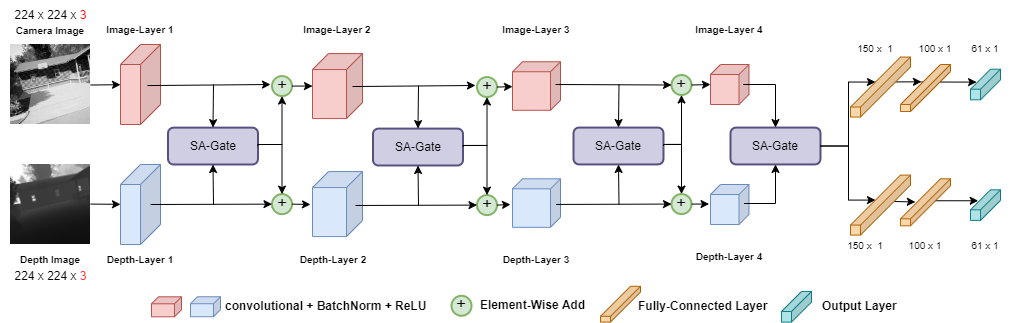
\includegraphics[scale=0.38]{./figure/2_method/SII2023_network_overall_2.png}
    \caption{Network Architecture. The training and test images were grayscaled to compress data size and speed up processing. However, when inference is used, the number of channels is 3 to make it a pre-trained ResNet input.}
    \label{fig:network_overall}
\end{figure*}

 \begin{figure*}[!t]
    \centering
    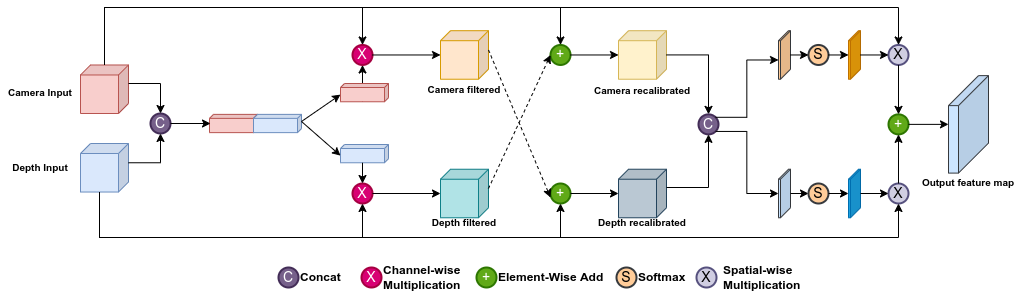
\includegraphics[scale=0.38]{./figure/2_method/sa_gate.png}
    \caption{SA-Gate Architecture}
    \label{fig:sagate_overall}
\end{figure*}

Ozaki proposed an attitude estimation method by extracting normal vectors from point clouds from LiDAR scan and integrating information from gyroscope and wheel odometry, based on the assumption that walls are mostly vertical to the horizontal plane in environments with artificial objects such as inside buildings\cite{ozaki_lidar_normal}. However, this approach is based on the assumption that there were many buildings and other human-made structures in the surrounding area. To solve this problem, he proposed a method to estimate the attitude using camera image and deep learning\cite{Ozaki_SII2021}. This method enables non-rule-based attitude estimation by training a numerical regression neural network with attitude data associated with camera images. Other methods exist to estimate the attitude by integrating the information from the gyroscope with the inference from the camera image using a numerical regression neural network\cite{ozaki_springer}. Attitude estimation from camera images using DNN, as in these methods, has the advantage of eliminating error accumulation. However, when the output layer is used as a numerical regression, the accuracy of the estimation is insufficient. This is due to the small number of parameters near the output layer, and the inadequacy of the expressive power of the numerical regression compared to the capability required for the attitude estimation task.

%尾崎は建物内などの人工物のある環境下では壁は水平面に対して鉛直であることがほとんどであるという前提のもと、LiDARから得られる点群から法線ベクトルを抽出、ジャイロスコープとホイールオドメトリからの情報を統合することでの姿勢推定手法を提案した。しかし、この手法は建物などの人工物が周囲に多数存在していることが前提であった。翌年彼は姿勢をカメラからの画像を深層学習を用いて推定する手法を提案した。この手法はカメラ画像と紐付けた姿勢のデータを数値回帰型のニューラルネットワークに学習させることでルールベースによらない姿勢推定を可能にするとともに、Monte-Carlo dropoutを用いることで深層学習の不確かさを推定することも可能にした。これらの手法のように、カメラ画像からDNNを用いてattitude estimationを行うことはerror accumulationがないといったメリットがある。しかし、output layerをnumerical regressionにした場合、estimationの精度は不十分であった。これはoutput layer付近のパラメータ数が少ないことが原因で、numerical regressionの持つ表現能力がattitude estimation taskに求められる能力に対して不十分であったことが原因であると考えられる

In our previous work, we achieved high attitude estimation accuracy by introducing a classification type output layer to neural network\cite{9708864} based on OCR method. But this method still has a problem with estimation accuracy in an unknown environment. To put camera attitude estimation using deep neural networks into practical use for a ground robot, it is necessary to improve the accuracy of attitude estimation in unknown environments. The key elements for this are a prior knowledge that the wall is vertical to the ground and the ground is horizontal, which played a key role in Ozaki's study\cite{ozaki_lidar_normal}, and sensors that can obtain this information. In this paper, the depth camera was adopted as a tool to obtain topographic information. Terrain information can also be obtained from LiDAR. However, the form of data obtained from LiDAR is very different from that of RGB images, making it a hard task to use as input for DNN\cite{ozaki_robosym}. In DNN, the integration of information from LiDAR and from the camera alone is a valid research project\cite{google_LiDAR_camera}. On the other hand, the depth image can be sampled with the same position, viewing angle, and size as the Image camera using equipment, enabling feature extraction where information from the camera image and information from the depth image interfere with each other.

%deep neural networkによるcamera attitude estimationを実用化するためにはunknown environmentでのattitude estimationの精度を向上する必要がある。これのために重要となる要素がOzakiのstudyでも重要な役割を果たした、壁は地面に対して垂直、地面は水平であるなどの事前知識と、それを情報として入手できるセンサである。地形の情報はLiDARからも入手することができる。しかし、LiDARは得られるデータの形態がRGB画像とは大きくかけ離れており、DNNのinputとするのには不適である。DNNにおいては、LiDARからの情報とカメラからの情報の統合だけでも一つの研究として成立する。その一方で、depth画像はIntel Realsenseなどの機器を用いればRGBカメラと同一の位置や視野角、サイズを持って画像を採取することが可能であり、RGB画像からの情報とdepth画像からの情報を相互に干渉し合う特徴量抽出を可能とする。

Feature extraction methods that intermingle information from camera and depth images have been used successfully in the field of semantic segmentation\cite{DBLP:journals/corr/abs-2011-06961}. These methods add information from the depth image as a supplement to the usual semantic segmentation. But Chen et al proposed a feature extraction method\cite{SAGATE} that interferes with information from the HHA image generated from the depth image and the camera image to improve segmentation accuracy and ensure the robustness of feature extraction. In this paper, to improve the accuracy of attitude estimation in unknown environments, the feature extraction module used in the method of Xing et al. is employed in the attitude estimation network. \par


%RGB画像とdepth画像、この2つから得られる情報を相互に干渉させながら特徴量抽出を行う手法はsemantic segmentationの分野で成功を収めている。これらの手法は通常のsemantic segmentationにdepth画像の情報を補助として加えるものであったが、Xingらはdepth画像から生成されるHHA画像とRGB画像からの情報を相互に干渉させて特徴量抽出を行う手法を提案し、segmentationの精度向上と特徴量抽出のロバスト性の確保を達成した。この論文では、未知環境での姿勢推定精度向上のために、Xingらの手法で用いられている特徴量抽出モジュールをattitude estimation networkに採用する

In this paper, we aim to improve the accuracy of attitude estimation in unknown environments by using different types of images as inputs: camera images for scenery and depth images for terrain information. The main contributions of this paper are as follows

%この論文では、風景画像を得られるcamera imageと地形情報を得られるdepth imageの異なる種類を持つ画像をinputとして、unknown環境におけるattitude estimationの精度改善を狙う。

\begin{itemize}
\item Highly accurate attitude estimation by introducing a feature extractor that can extract both topographic and landscape information.
\item Improved accuracy of attitude estimation in unknown environments in simulators.
\item Effectiveness of the classification type output layer in the task of estimating the attitude.
\end{itemize}

\section{Proposed Method}

\subsection{Network}
The network used in the experiment is shown in Fig.\ref{fig:network_overall}.
The two main features of this method are a classification type output layer based on OCR methods and a camera-depth feature extractor based on the success in semantic segmentation.

%本手法では, OCRの手法を参考にしたclassification type output layerと, semantic segmentationでの成功を参考にしたRGB-D feature extractorの2つを大きな特徴とする。

\subsubsection{Camera-Depth Feature Extractor}
The feature extractor called SA-Gate used in this method\cite{SAGATE} is originally proposed by Chen et al. for semantic segmentation. SA-Gate's structure is shown in Fig.\ref{fig:sagate_overall}. As shown in Fig.\ref{fig:network_overall}, the feature extractor in this method uses the camera image and depth image as inputs and inputs the feature map obtained through the convolution layer to a special module called SA-Gate. The role of SA-Gate is to mitigate the influence of noise that inevitably gets mixed into the camera and depth image. In addition, SA-Gate has the role of recalibrating the two types of modalities from the camera image and the depth image and fusing the complementary information. The resulting feature map can be used as an input to the network for feature extraction that is more robust to noise. The parameter of the convolution layer of the feature extractor in this method is the pre-trained weight of ResNet\cite{he2015deep}, which enables efficient training and high classification ability.

%本手法で用いるfeature extractorは、semantic segmentationのためにChenらの研究で提案されたものを使用する。図AAAの通り、本手法のfeature extractorはcamera Imageとdepth imageの2つをinputとして、convolutional layerを通して得られたfeature mapをSA-Gateと言う特殊なモジュールへ入力する。このSA-Gateの役割はdepth画像にどうしても混入してしまうノイズ影響を緩和することに大きな効果がある。この他にも、SA-Gateにはcamera imageとdepth imageから来るtwo type modalitiesをrecalibrateしてcomplementary informationをfuseする役割を持つ、これによって得られたfeature mapをnetworkのinputとすることでよりノイズにロバストなfeature extractionを可能とする。本手法におけるfeature extractorのconvolutional layerのパラメータはResNetのpretrained weightを使用した。ResNetのpretrained weightを使用することで効率的な学習と高い識別能力を獲得することができた。

\begin{figure}[thpb]
\centering
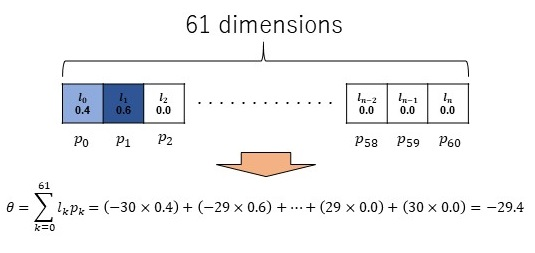
\includegraphics[scale=0.5]{./figure/2_method/classification_layer.jpg}
\caption{Classification Type Output Layer}
\label{fig:classification_layer}
\end{figure}

\subsubsection{Classification Type Output Layer}
In a previous study, we achieved high accuracy in attitude estimation by introducing a classification type network\cite{9708864}, which has shown high performance in the field of OCR\cite{kuzushiji_dl}, to the attitude estimation task. Handwritten characters vary greatly in form depending on the writer and the period in which they were written. However, the network equipped with a classification type output layer shown in Fig.\ref{fig:classification_layer} has acquired a high recognition ability. In addition, the landscape image captured by the camera differs greatly depending on the location, even at the same angle of orientation. In a previous study, we found commonalities between two different types of tasks in this location and introduced a classification type network for the attitude estimation task. The results showed that the classification type network had the best accuracy in terms of attitude estimation accuracy compared to the existing numerical regression type network.

The output layer of the classification type is limited in the range of angles it handles, unlike the numerical regression type, but within that range, it can perform high recognition ability. This is because cross-entropy loss is introduced during training. Cross-entropy loss provides the benefits of the theory of maximum likelihood estimation that enables efficient Bayesian inference by specifying a conjugate prior.

The experiments in this paper deal with angles from -30 to +30 degrees. Since this method is designed to be mounted on a robot in Fig.\ref{fig:CCV}, it does not have the same problems as drones even if the angles to be handled are limited. In this paper, the classification type output layer has 61 dimensions. This is the result of assigning the corresponding index to each angle, such as index 0 for -30 degrees, index 1 for -29 degrees, and so on. Each index expresses the probability of an angle within the range of 0 to 1. For example, if an angle of -29.40[deg] is to be represented as the correct answer label in the class identification network, the 0th index assigned as -30.0 degrees is assigned a value of 0.40, and the 1st index assigned as -29.0 degrees is assigned a value of 0.60. In this way, the output layer of the class identification neural network, which can only represent values from 0.0 to 1.0, can also represent values from -30.0 to 30.0.

%以前の研究で我々はOCRの分野で高い性能を発揮しているclassification type networkをattitude estimationタスクに導入することで高いattitude estimation accuracyを達成した。手書きの文字は書く人や書かれた時代によって字の形は大きく異る。しかし、classification type output layerを備えたネットワークで学習することで高い識別能力を獲得している。また、カメラ画像についても同じ姿勢角であっても場所によって撮影される風景画像は大きく異る。以前の研究において、我々はこの箇所に2つの異なる種類のタスク間での共通性を見出し、attitude estimation taskにclassification type networkを導入した。この結果、classification type networkのattitude estimation accurcyは既存のnumerical regression type networkと比較して最も良い精度であった。

%classification typeの出力層は扱う角度の範囲はnumerical regression typeとは異なり限定されるが、その範囲内では高い識別能力を持っている。これは学習時にcross entropy lossを導入しているためである。クロスエントロピー損失は、共役事前分布を指定することで効率的なベイズ推定を可能にするという最尤推定の理論の利点を提供する。

%本論文での実験では、-30度から+30度までの角度を扱う。本手法はAAAAAのようなロボットにおいて搭載することを前提としているため、扱う角度が限定されてもドローンのような問題は発生しない。本論文においてclassification type output layerは61次元を取る。これは-30度にはインデックス0、-29度にはインデックス1といったように角度に応じて対応するインデックスを割り振っていった結果である。それぞれのインデックスは0から1までの範囲内で角度の確率を表現する。例えば-29.55[deg]という角度をクラス識別ネットワークの正解ラベルとして表現したい場合、-30.0度として割り振られた0番目のインデックスには0.55、-29.0度として割り振られた1番目のインデックスには0.45の値をそれぞれ割り振る。このようにすることで0.0から1.0までしか表現できないクラス識別ニューラルネットワークの出力層でも-30.0から30.0までの値を表現することができる。


\subsection{Random Window Method for Input Image}\label{sec:random_window}
In this method, the center position of the input image is randomly selected, and inference is performed using multiple images cropped from the center of the image, which is also used in OCR methods\cite{OCR_paper}. The probability distribution obtained by inference using multiple images clipped at a randomly selected center position is different each time. These are averaged to compensate for the inference error. Such clipped images are used not only for inference but also for generating training data.

%本手法ではOCRの手法でも用いられている、入力画像に対して中心位置をランダムに選び、そこを中心に切り抜かれた画像を複数枚用いて推論を行う。中心位置をランダムに選択して切り抜いた複数枚の画像を用いて推論すると得られる確率分布は毎回異なるものが得られる。これらを平均することで推論の誤差をcompensateしている。このような画像の切り抜きは推論のときだけでなく、学習用データの生成時にも使用される。

\begin{figure}[thpb]
\centering
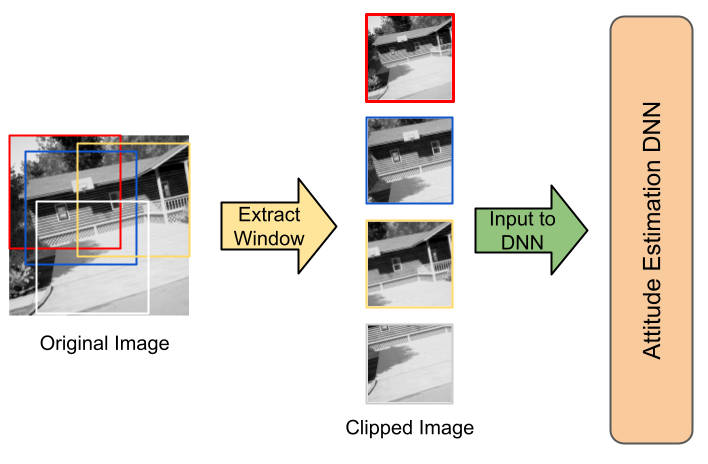
\includegraphics[scale=0.4]{./figure/2_method/RandomWindow_2.png}
\caption{Extraction Windows from Original Camera Image.}
\label{fig:extract_windows}
\end{figure}

\section{Experiment Environment}

\begin{figure}[htbp]
\centering
  \begin{minipage}[h]{0.45\linewidth}
    \centering
    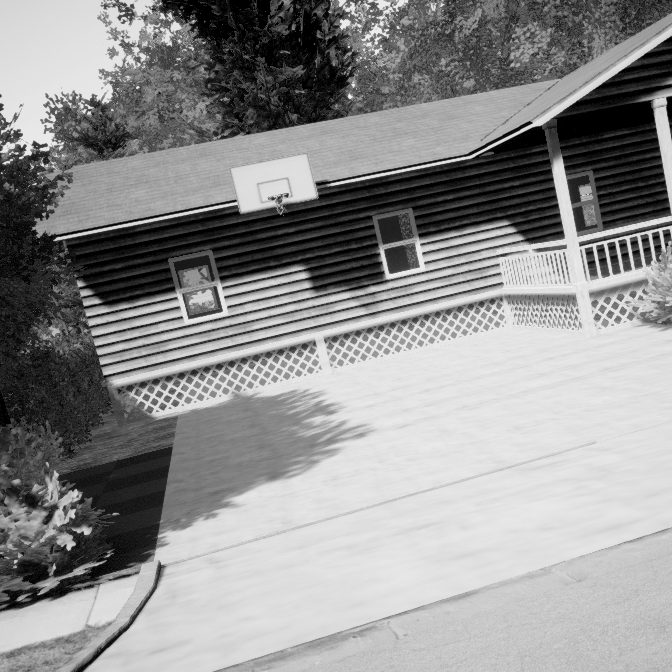
\includegraphics[keepaspectratio, scale=0.11]{./figure/3_environment/image10_0.png}
    \subcaption{Camera Image}\label{fig:known_env_image}
  \end{minipage} 
  \begin{minipage}[h]{0.45\linewidth}
    \centering
    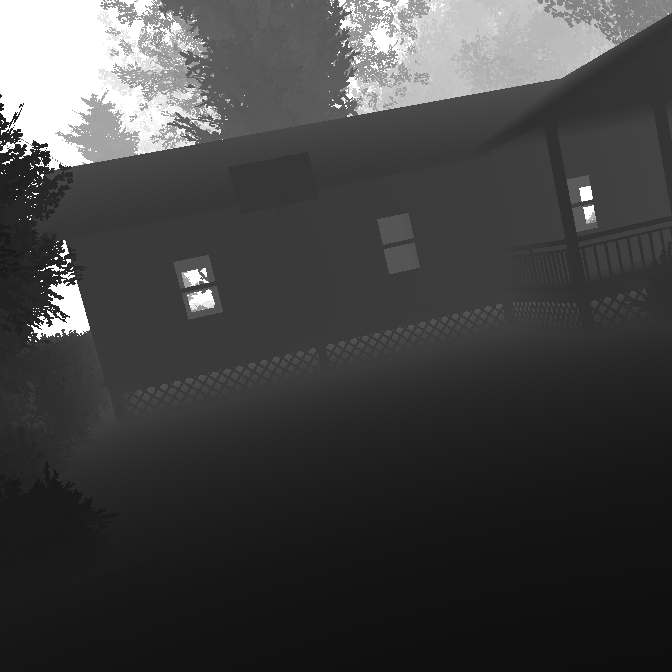
\includegraphics[keepaspectratio, scale=0.11]{./figure/3_environment/depth10_0.png}
    \subcaption{Depth Image}
  \end{minipage}
  \caption{Images Obtained from the Known Environment}\label{fig:known_env}
\end{figure}

\begin{figure}[thpb]
\centering
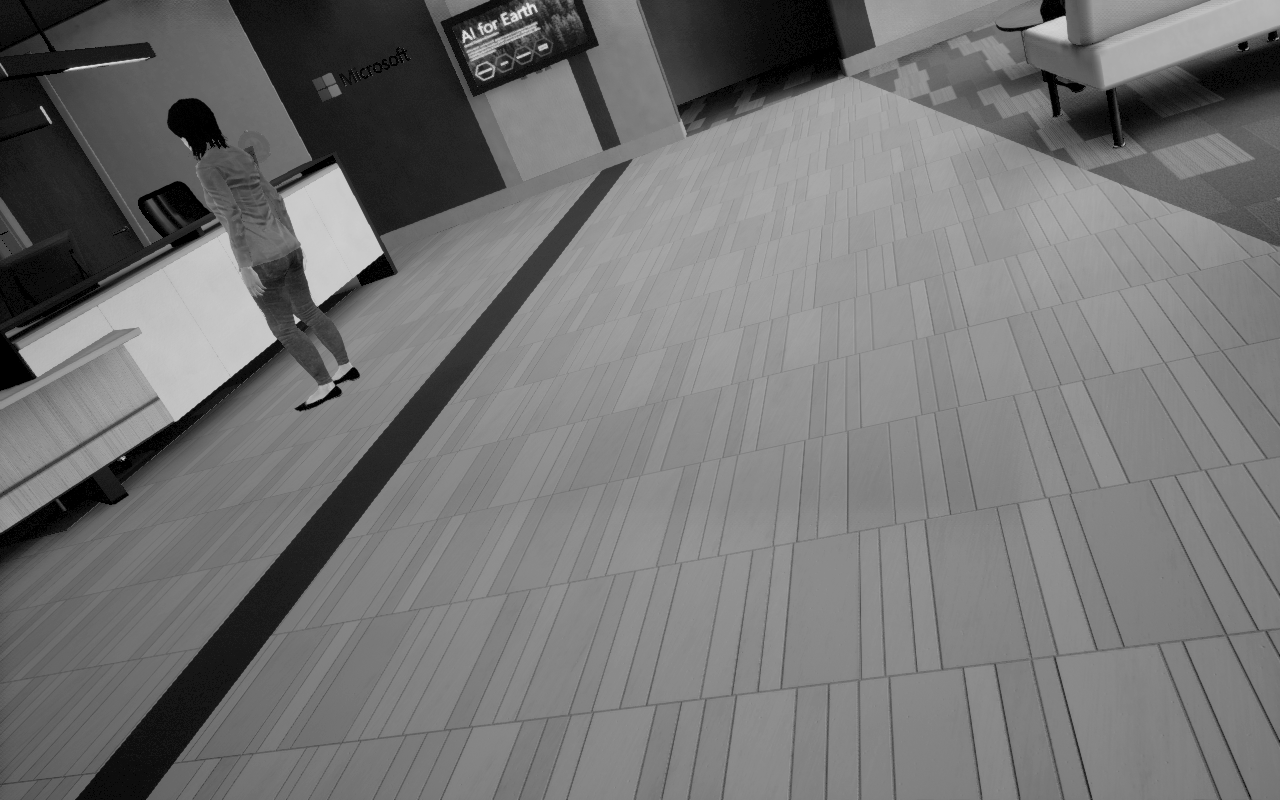
\includegraphics[scale=0.08]{./figure/3_environment/image64.png}
\caption{Image Obtained in Unknown Environment}
\label{fig:unknown_env}
\end{figure}

\subsection{Dataset Collection}\label{sec:dataset}
Microsoft AirSim\cite{airsim_paper} was used to collect data. This software is a drone simulator, but it can collect various data related to the task of attitude estimation, such as depth image collection. The drone spawned at random locations and collected images and attitude data as seen from those locations. To maximize the effectiveness of the method described in Sec.\ref{sec:random_window}, we modified the method to collect about five small images from a single location. In addition, images were collected from two environments for data collection. One environment was a suburban residential area with a moderate presence of trees and buildings. The images obtained in this environment were used for training and validation data and as part of the test data. The other environment was a Microsoft office building. Images obtained from this environment were not used for training data at all but were used as test data to measure performance in the environment in which the findings were obtained. Based on the above rules, 150,000 pairs of camera and depth images for training, 25,000 pairs for validation, and 1,000 pairs for testing were collected from the residential area environment described above. In addition, 1,000 pairs were collected from the office building environment described above for testing in the findings environment. The environment used to collect data for training is shown in Fig.\ref{fig:known_env}, and the environment used to collect data in an unknown environment is shown in Fig.\ref{fig:unknown_env}. The training and test images were grayscaled to compress data size and speed up processing. However, when inference is used, the number of channels is 3 to make it a pre-trained ResNet input. In a real environment, images obtained from a depth camera are subject to significant noise. However, in this study, in order to verify the effectiveness of using both the camera image and the depth image, we decided not to add noise information in the simulator environment. When trying to collect image and attitude data in a real environment, there is the problem of difficulty in obtaining accurate attitude values. Therefore, this experiment was conducted only in the simulator environment.

%データセットの収集にはMicrosoft AirSimを使用した。このソフトはドローンのシミュレータであるが, depth画像の採取などattitude estimationのタスクに関わる様々なデータが採取できる。実験データの採取では、ドローンをランダムな位置にスポーンさせてその位置から見たcamera imageとdepth image、そしてattitude dataを採取する方法を取った。また、Sec. AAAで紹介した手法の効果を最大限高めるため、一つの地点から小画像を5枚ほど採取するように変更した。また、データ採取にあたって2つの環境から画像を採取した。一つは郊外の住宅街をもした環境であり、木や建物などが適度に存在する。この環境下で得られた画像はtrainとvalidation用のデータと、testデータの一部に使用した。もう一つはマイクロソフト社のオフィスビルをもした環境であり、この環境から得られた画像は訓練用データには一切使用せず、所見の環境でのパフォーマンスを図るtest用のデータとして使用した。以上のルールに基づいて、訓練用のcamera imageとdepth imageを15万ペア、validation用として5万ペア、test用として1000ペアを先述の住宅街の環境から採取した。また、所見の環境でのテストのために先述のオフィスビルの環境から1000ペアを採取した。データサイズの圧縮と、処理の高速化のために訓練用の画像とテスト用の画像はグレイスケール化を行った.ただし、inferenceの時はpretrainedなResNetのinputとするためにチャネル数を3で読み込む.実環境においてdepthカメラから得られる画像には大きなノイズが発生する。しかし、本研究においてはcamera imageとdepth imageの2つを使うことの有効性を検証するために、シミュレータ環境におけるノイズ情報は付与しないことにした。


\subsection{Hardware}
%i9-10900K 32GB RTX2080Ti
%Nvidia DGX1
In this experiment, different hardware was used for learning and inference. We used NVIDIA DGX-1 for training, Intel core i9-10900K 10 cores 20 threads, 32GB RAM, and GeForce NVIDIA RTX2080Ti GPU for inference.

%今回の実験では学習と推論で異なるハードウェアを使用した。学習にはNvidia社製のDGX1を使用、推論にはIntel core i9-10900K 10コア20スレッド、RAMは32GB、GPUにはNvidia RTX2080Tiを使用した。




\subsection{Comparison Method}
Kawai's method\cite{9708864} and Ozaki's method\cite{Ozaki_SII2021} (MLE, Regression) were trained and tested as comparison methods. To examine the effect of the SA-Gate, we trained and tested a network without the SA-Gate from the network with the best experimental results in the proposed method in sec.\ref{sec:result}.

\begin{table}[htbp]
\begin{center}
\caption{Training Parameter}
  \begin{tabular}{c|c} \hline
    Parameter & Value \\ \hline
    Learning Loss & 1e-4 \\
    Mean Element & 0.5 \\
    Std Element & 0.5 \\
    Epochs & 50 \\
    Batch Size & 256 \\
    Dropout Rate & 0.1 \\
    L2 Regularization Alpha & 5e-5 \\
    Optimizer & Adam \\
    Loss Function & Cross Entropy Loss \\ \hline
  \end{tabular}
  \label{tab:Training_Parameter}
\end{center}
\end{table}

\subsection{Train Network}
The hyperparameters used in the train are shown in Tab.\ref{tab:Training_Parameter}. During training, 8 GPUs were parallelized for training. Pytorch is used for the implementation. The feature extractor in the proposed method can be equipped with ResNet of any layer depth. ResNet was trained using 18, 34, 50, 101, and 152 as feature extractor, respectively. It took about 50 hours to complete the training. 
%Train is shown in Fig\ref{fig:train_network}.

%提案手法におけるfeature extractorは任意の層の深さのResNetを搭載することができる。本実験ではResNet18, 34, 50, 101, 152それぞれで学習を行い、推論試験を行った。Training graphを図AAAAに示す。学習が終了するまでの時間は概ね50時間ほどであった。



\section{Experiment Result}

\begin{table*}[!t]
\centering
\caption{MAE of Estimated Attitude}\label{tab:MAE_of_Error}
\begin{tabular}{|cl|rr|rr|r|}
\hline
\rowcolor[HTML]{C0C0C0} 
\multicolumn{2}{|c|}{\cellcolor[HTML]{C0C0C0}}                                                                                    & \multicolumn{2}{c|}{\cellcolor[HTML]{C0C0C0}\begin{tabular}[c]{@{}c@{}}Inference in \\ Training Environment\end{tabular}}                                                                                                    & \multicolumn{2}{c|}{\cellcolor[HTML]{C0C0C0}\begin{tabular}[c]{@{}c@{}}Inference in \\ Unknown Environment\end{tabular}}                                                                                                     & \multicolumn{1}{c|}{\cellcolor[HTML]{C0C0C0}}                                                                                   \\ \cline{3-6}
\rowcolor[HTML]{C0C0C0} 
\multicolumn{2}{|c|}{\multirow{-2}{*}{\cellcolor[HTML]{C0C0C0}Method Name}}                                                       & \multicolumn{1}{c|}{\cellcolor[HTML]{C0C0C0}\begin{tabular}[c]{@{}c@{}}MAE of\\ Roll {[}deg{]}\end{tabular}} & \multicolumn{1}{c|}{\cellcolor[HTML]{C0C0C0}\begin{tabular}[c]{@{}c@{}}MAE of\\ Pitch {[}deg{]}\end{tabular}} & \multicolumn{1}{c|}{\cellcolor[HTML]{C0C0C0}\begin{tabular}[c]{@{}c@{}}MAE of\\ Roll {[}deg{]}\end{tabular}} & \multicolumn{1}{c|}{\cellcolor[HTML]{C0C0C0}\begin{tabular}[c]{@{}c@{}}MAE of\\ Pitch {[}deg{]}\end{tabular}} & \multicolumn{1}{c|}{\multirow{-2}{*}{\cellcolor[HTML]{C0C0C0}\begin{tabular}[c]{@{}c@{}}Inference\\ Time {[}s{]}\end{tabular}}} \\ \hline
\multicolumn{1}{|c|}{}                                                                               & ResNet18                   & \multicolumn{1}{r|}{1.6887}                                                                                  & 1.5555                                                                                                        & \multicolumn{1}{r|}{4.5271}                                                                                  & 9.0285                                                                                                        & 0.020                                                                                                                           \\ \cline{2-7} 
\multicolumn{1}{|c|}{}                                                                               & ResNet34                   & \multicolumn{1}{r|}{1.7674}                                                                                  & 1.8037                                                                                                        & \multicolumn{1}{r|}{4.0867}                                                                                  & 8.3678                                                                                                        & 0.025                                                                                                                           \\ \cline{2-7} 
\multicolumn{1}{|c|}{}                                                                               & ResNet50                   & \multicolumn{1}{r|}{\textbf{1.5245}}                                                                         & \textbf{1.5183}                                                                                               & \multicolumn{1}{r|}{\textbf{3.5384}}                                                                         & \textbf{7.8504}                                                                                               & 0.027                                                                                                                           \\ \cline{2-7} 
\multicolumn{1}{|c|}{}                                                                               & ResNet101                  & \multicolumn{1}{r|}{2.2452}                                                                                  & 1.9573                                                                                                        & \multicolumn{1}{r|}{4.3105}                                                                                  & 8.0860                                                                                                        & 0.036                                                                                                                           \\ \cline{2-7} 
\multicolumn{1}{|c|}{\multirow{-5}{*}{\begin{tabular}[c]{@{}c@{}}Proposed\\ Method\end{tabular}}}    & ResNet152                  & \multicolumn{1}{r|}{1.6938}                                                                                  & 1.9545                                                                                                        & \multicolumn{1}{r|}{3.8817}                                                                                  & 9.3533                                                                                                        & 0.050                                                                                                                           \\ \hline
\multicolumn{1}{|c|}{}                                                                               & Kawai's Method             & \multicolumn{1}{r|}{2.2345}                                                                                  & 2.2633                                                                                                        & \multicolumn{1}{r|}{4.5705}                                                                                  & 12.6040                                                                                                       & 0.010                                                                                                                           \\ \cline{2-7} 
\multicolumn{1}{|c|}{}                                                                               & Ozaki's Method(MLE)        & \multicolumn{1}{r|}{11.7984}                                                                                 & 12.5593                                                                                                       & \multicolumn{1}{r|}{14.4135}                                                                                 & 15.3828                                                                                                       & 0.005                                                                                                                           \\ \cline{2-7} 
\multicolumn{1}{|c|}{\multirow{-3}{*}{\begin{tabular}[c]{@{}c@{}}Camera \\ Image Only\end{tabular}}} & Ozaki's Method(Regression) & \multicolumn{1}{r|}{9.5726}                                                                                  & 7.6709                                                                                                        & \multicolumn{1}{r|}{9.2231}                                                                                  & 14.8570                                                                                                       & 0.005                                                                                                                           \\ \hline
\multicolumn{1}{|c|}{W/O SA-Gate}                                                                    & ResNet50                   & \multicolumn{1}{r|}{1.9692}                                                                                  & 1.7023                                                                                                        & \multicolumn{1}{r|}{4.5331}                                                                                  & 7.3232                                                                                                        & 0.029                                                                                                                           \\ \hline
\end{tabular}
\end{table*}
\subsection{Inference in Known and Unknown Environment}\label{sec:result}
To verify the performance of the network, inferences were tested under the same environment as the training data and the environment of the findings, respectively. The generation of the small windows described in Sec.\ref{sec:random_window} was set up to generate 15 windows. The inference time in the table showing the experimental results is the inference time per window. The number of windows was set to 15 in this experiment in consideration of the balance between estimation time and accuracy.

%ネットワークの性能を確かめるために、訓練データと同じ環境と所見の環境のもとでそれぞれ推論の試験を行った。実験の結果を表AAAAAに示す。表AAAAの中にあるMAEとは、数多くの枚数があるテストデータ中で、一枚一枚推論の試験をしていく中で、真の値と推論の値の誤差を加算して最終的に平均値として算出した値である。AAAAA節で述べた小さい窓の生成は15枚を生成するように設定した。実験結果を示す表にある推論時間は窓1枚あたりの推論時間である。窓の枚数を増やすことでattitude estimationの精度を向上させることが可能であるがそれに合わせて推定時間は増大する、推定時間と精度のバランスを考慮して本実験では窓の枚数を15枚と設定した。


The results of the experiment are shown in Tab.\ref{tab:MAE_of_Error}. The MAE in Tab.\ref{tab:MAE_of_Error} is the value calculated by adding up the errors between the true value and the estimated value in the course of testing the inference for each piece of test data, of which there are numerous pieces, and finally calculating the average value. The inference test results show that the proposed method, which uses the camera image and the depth image as two inputs, has the best inference accuracy. Among the proposed methods, the smallest error value was obtained when ResNet50 was set as the feature extractor. In an unknown environment, all conventional methods using only the camera image have low accuracy in attitude estimation, but the proposed method using both the camera image and the depth image as inputs has better accuracy than conventional methods. However, the proposed method, which uses both the camera image and the depth image as inputs, shows better accuracy than the conventional methods. However, the proposed method, which uses both camera and depth images as inputs, showed better accuracy than the conventional methods. However, the accuracy of these attitude estimation methods is still low considering that they are used on a robot such as the one shown in Fig.\ref{fig:CCV}. To investigate the effect of the SA-Gate, training and inference tests were conducted on the network of the proposed method without the SA-Gate, and ResNet50, which showed the best accuracy in the aforementioned tests, was used as the feature extractor. The results showed that the network without SA-Gate was less accurate than the network with SA-Gate in all values except for the pitch in an unknown environment.

%推論テストの結果、カメラ画像とdepth imageの2つをinputとする提案手法が最も良い推論精度を発揮した。提案手法の中でも、ResNet50をfeature extractorとして設定した時の誤差が最も小さい値となった。unknown environmentにおいて、camera imageのみを用いる従来手法はすべて低いattitude estimation accuracyであったが、camera imageとdepth imageの2つをinputとする提案手法は従来手法より優れた精度を発揮した。しかし、これらのattitude estimation accuracyは図AAAAのようなロボットに搭載することを考えると依然低いaccuracyであった。

%SA-Gateの効果を調べるため、提案手法のネットワークからSA-Gateを抜いたものを用意して学習と推論試験を行った。feature extractorには先程述べた試験において最も優れた精度であったResNet50を用いた。試験の結果、SA-Gate抜きのネットワークはunknown environmentにおけるpitchを除いて全ての値においてSA-Gate有りより精度が低かった。

\subsection{Consideration}\label{sec:consideration}
This method demonstrated the best accuracy in the attitude estimation task in an unknown environment. However, even with this method, many issues remain in practical use. One of the possible reasons for the improvement in accuracy compared to the conventional method is the introduction of SA-Gate, which obtains a feature map by aligning the information obtained from the camera image and the depth image while mutually interfering with each other. The high-quality feature map obtained by this method is considered to have contributed to the improvement of the accuracy of the attitude estimation in unknown environments.

%本手法はunknown environmentにおけるattitude estimation taskにおいて最も優れた精度を発揮した。しかし、それを持ってしても実用面では多くの課題が残る結果となってしまった。従来手法と比較してaccuracyが向上した要因として考えられるのがSA-Gateの導入である。SA-Gateはcamera imageとdepth imageから得られる情報を相互に干渉させながらalignさせてfeature mapを入手する。この手法によって得られる質の高いfeature mapがunknown environmentにおけるattitude estimation accuracyの向上に寄与したと考えられる。

In conventional methods, when a network has data with different modality (e.g., camera image and depth image) as inputs, it is common to concatenate the resulting feature maps\cite{ozaki_robosym}\cite{SAGATE}\cite{RGBD_1}\cite{RGBD_2}. While such methods, including the proposed method, can improve accuracy compared to the case of using only camera images, the structure of the network becomes more complex, increasing computational cost. However, the accuracy did not improve that much in response to the increased processing burden, and this has become a problem in the practical application of networks with cross-modality information as input. We believe that the method using attention in this method\cite{google_LiDAR_camera} may be effective for such tasks that require multiple types of data as input. It is also pointed out that a decision tree has better classification ability than a neural network in the problem of tabular data classification\cite{DL_isnot}. The proposed method, which uses two types of data as inputs and a classification-type output layer, be a good match for such a method.

%従来までの手法では、camera imageとdepth imageなど異なるmodalityを持つデータをinputとするネットワークでは得られたfeature mapをconcatするやり方が一般であった。提案手法を含めて、このような方法はcamera imageのみの場合と比べて精度を向上させることができる半面、ネットワークの構造は複雑になりcomputational costの増大を招いた。しかし、そのような処理負担の増大に対して精度の向上はそこまで多くなく、cross modalityな情報をinputとするネットワークを実用化する際の問題点となってしまった。


In the unknown environment, the accuracy of pitch estimation was lower than that of roll estimation. Although this method estimates the attitude based on the scenery in the image, the nature of the changes that appear in the image is different when the roll value is changed and when the pitch value is changed. 
Taking the image shown in Fig.\ref{fig:known_env_image} as an example, changing the roll will greatly change the way house and window appear in the image, such as by changing the tilt angle. However, the pitch does not change the tilt, but rather the range of the landscape in the image; in the case of Fig.\ref{fig:known_env_image}, when the angle of the pitch is closer to 0 degrees, the window is more likely to appear in the center of the image, and this also happens when the height of the camera is increased. Unlike roll, pitch was not a sole factor in determining the appearance of the landscape image, which may have been the result of poor pitch accuracy. This suggests that the pitch estimation accuracy was low in the unknown environment, and at the same time, when the network made the attitude estimation, it was based on the reflection of objects that were built vertically to the ground, such as people, furniture, and buildings. The network without SA-Gate had lower accuracy in pitch estimation under unknown environment than the network with SA-Gate, but this may be due to the fact that the network could not fully learn the change of scenery caused by pitch changes even with SA-Gate.

%unknown environmentにおいて、pitchの推定精度はrollでの精度よりも低い値となった。本手法は画像に映る風景をもとにattitudeを推定しているが、rollの値が変わった場合とpitchの値が変わった場合では画像に現れる変化の性質が異なる。Fig.AAAのような画像を例にとると、rollを変更した場合は人やテーブルの傾き角度が変わるなど映り方が大きく変わる。しかし、pitchの場合はこのような傾き方の変更ではなく画像に映る風景の範囲が変わる。pitchの角度を0度に近づけたとき、窓は画像の中央に映りやすくなるが、これはカメラの高さを高くしても同様のことが起きる。rollと異なり、pitchが風景画像の映り方を決める決定的な要素にならなかったのがpitchの精度が悪かった結果であると考えられる。このことからunknown environmentにおいてpitchの推定精度が低かったと考えられ、同時にネットワークがattitude estimationをする際は人や家具、建物など、地面に対して鉛直に建てられている物体の映り方を参考にしていると考えられる。SA-Gateなしのネットワークの方が, ありのものと比べてunknown環境下でのpitch推定精度が低かったが、これはSA-Gateを用いてもネットワークがpitchの変化による風景の変化を学習しきれなかったことが原因と考えられる.

\section{Conclusion}
With this paper, we have shown that the attitude estimation method using camera images and depth images leads to improved accuracy in unknown environments. The method of combining camera and depth images has been shown to be effective in segmentation tasks, but this paper confirms that it is also effective in the field of attitude estimation.

%本論文によって、カメラ画像と深度画像を用いたattitude推定手法はunknown環境において精度向上につながることを示した。これまでカメラ画像と深度画像を組み合わせる手法はセグメンテーションのタスクなどでは存在し有効性を示していたが、本論文によってそれがattitude推定の分野においても有効であることが確認された。


In this paper, a rather complex mechanism is introduced into the network to extract mutually interfering information from the depth and camera images, including the introduction of SA-Gate. Although it was able to achieve the desired effect, the complexity of the network led to a large increase in computational cost and processing time compared to the conventional method. Therefore, in order to put this method into practical use, it is necessary to improve it from various directions, such as revising the calculation method and enhancing the calculation capacity.

%本論文ではSA-Gateの導入など、深度画像とカメラ画像からの相互干渉し合う情報を抽出するためにやや複雑な機構をネットワークに導入した。それによって目的通りの効果を発揮することができたものの、ネットワークの複雑化は計算コストと処理時間の大きな増加を招き、従来手法と比べて処理時間は大きく増加した。したがって、本手法を実用化するにあたっては計算方法の見直しや計算能力の強化など、さまざまな方向からの改良が必要となる。

The proposed method demonstrated superior accuracy in attitude estimation in an unknown environment compared to conventional methods. In the future, we aim to develop a method that can perform more advanced attitude estimation for use with robots.

%提案手法はunknown environmentにおいて従来手法と比較して優れたattitude estimation accuracyを発揮した。今後はロボットへの搭載を前提としてより高度なattitude estimationを行える手法の開発発展を目指す。



\section{Appendix}\label{sec:appendix}
\begin{comment}
\subsection{MAE of Attitude Estimation}
The results of inference are presented in Sec.\ref{sec:result} as Tab.\ref{tab:MAE_of_Error}. In this section, we present a scatterplot in Fig.\ref{fig:MAE_scatter} showing the error between the networks that performed well in the proposed method and the inference results of the comparison method. As shown in Fig.\ref{fig:MAE_scatter} and Fig.\ref{fig:MAE_scatter_unknown}, the points showing the inference results of the proposed method using the depth image are concentrated near the origin. This indicates that the use of the depth image is effective in attitude estimation. Fig.\ref{fig:MAE_scatter_unknown}, which shows the estimation results in an unknown environment, shows that the network with SA-Gate has the best accuracy in the estimation of roll. On the other hand, the network without SA-Gate was more accurate in pitch estimation.
\end{comment}

\subsection{In the Attitude estimation task, where does the network focus its attention?}
To understand where the network is focusing its attention in the attention estimation task, we used Grad-CAM\cite{Grad-CAM} in Kawai's method\cite{9708864} to determine where the feature map was obtained from the attention. Since Grad-CAM supports only one input network, existing methods were used instead of the network of the proposed method. Some images processed by Grad-CAM are shown in Fig.\ref{fig:grad_cam}. As can be seen from these two figures, in the attitude estimation, the network directs its attention to the shape of the buildings and columns in the image. Buildings, columns, and beams as seen in the image are perpendicular or horizontal to the ground. This information is obtained by the network in the training process and is used in the attitude estimation process. This trend is particularly pronounced in the roll estimation and is visualized in Fig.\ref{fig:roll_example}. This indicates that for the attitude estimation in DNN using camera images, landmark objects are necessary, as in the method of Ozaki\cite{ozaki_lidar_normal}. However, compared to the LiDAR-based attitude estimation, the camera image-based estimation requires only a landmark object in front of the robot, so there are fewer restrictions on the environment in which it can demonstrate its capabilities.




%Attitude estimation taskにおいて、ネットワークはどこを注目しているのかを把握するため、Kawaiの手法においてGrad-CAMを使用してfeature mapがどこを注目して得られたものなのかを可視化した。Grad-CAMは1入力のネットワークにしか対応していないため、提案手法のネットワークではなく既存の手法を用いた。この2つの図からわかるように、attitude estimationにおいてネットワークは画像の中にある建物や柱の形状にattentionを向けていることがわかる。画像に現れるような建物や柱、梁の形状は地面に対して垂直ないし水平である。この情報をネットワークは学習の中でつかんでおり、attitude estimationのときに役立てている。とくにrollの推定においてこの傾向は顕著であり、図CCCCCにもその様子が可視化されている。このことから、カメラ画像によるDNNでのattitude estimationにおいては、尾崎らの手法と同じくランドマークとなる物体が必要であることがわかる。ただし、LiDARを用いたattitude estimationと比較して、camera imageによる推定ではロボットの前方にランドマークとなる物体があればよいので、能力を発揮できる環境の制約は少ない。

\begin{comment}
\subsection{Source Code}
The source code used in the experiments is as follows. The source code can be downloaded from the following link.

%実験の際に使用されたソースコードは以下の通りである。機会学習のコードの場合、以下のリンクから訓練済みモデルもダウンロードできる。

\begin{itemize}
    \item Source code for proposed and comparison method. It is implemented using Python and Pytorch and Docker.
    \url{https://github.com/Hibiki1020/camera_and_depth_image_attitude_estimator}
    \item Source code for collect data. It is implemented using C++ and AirSim and Unreal Engine API.
    \url{https://github.com/Hibiki1020/RGBD_LiDAR_airsim_controller}
\end{itemize}

\end{comment}

\section{Acknowledgement}
We have received generous support from new Energy and Industrial Technology Development Organization (NEDO) and Meiji University Research Cluster for Autonomous Robotic Systems for study. We would like thank it.

\addtolength{\textheight}{-12cm}   % This command serves to balance the column lengths
                                  % on the last page of the document manually. It shortens
                                  % the textheight of the last page by a suitable amount.
                                  % This command does not take effect until the next page
                                  % so it should come on the page before the last. Make
                                  % sure that you do not shorten the textheight too much.

%%%%%%%%%%%%%%%%%%%%%%%%%%%%%%%%%%%%%%%%%%%%%%%%%%%%%%%%%%%%%%%%%%%%%%%%%%%%%%%%



%%%%%%%%%%%%%%%%%%%%%%%%%%%%%%%%%%%%%%%%%%%%%%%%%%%%%%%%%%%%%%%%%%%%%%%%%%%%%%%%



%%%%%%%%%%%%%%%%%%%%%%%%%%%%%%%%%%%%%%%%%%%%%%%%%%%%%%%%%%%%%%%%%%%%%%%%%%%%%%%%


\bibliography{reference} %hoge.bibから拡張子を外した名前
\bibliographystyle{unsrt} %参考文献出力スタイル

\newpage

\begin{figure}[htpb]
\centering
  \begin{minipage}[htpb]{1.0\linewidth}
    \centering
    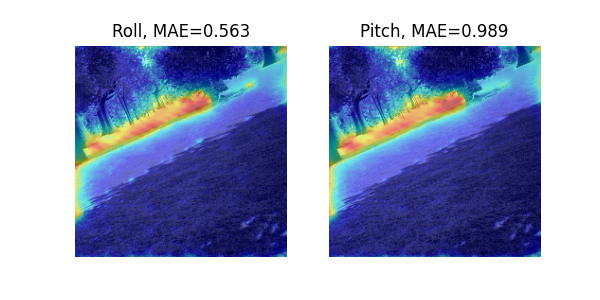
\includegraphics[keepaspectratio, scale=0.55]{./figure/appendix/known_env/image_12.png}
    \subcaption{Image Obtained from Forest in Known Environment}
  \end{minipage} \\
  \begin{minipage}[htpb]{1.0\linewidth}
    \centering
    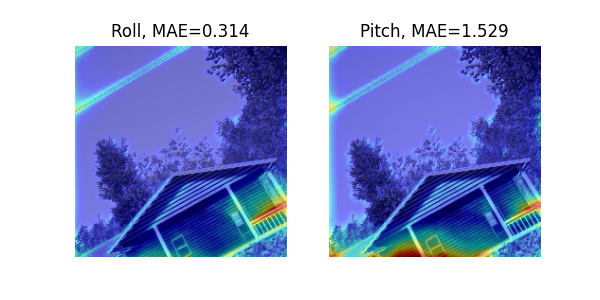
\includegraphics[keepaspectratio, scale=0.55]{./figure/appendix/known_env/image_35.png}
    \subcaption{Image Obtained from House in Known Environment}
  \end{minipage} \\
\centering
  \begin{minipage}[htpb]{1.0\linewidth}
    \centering
    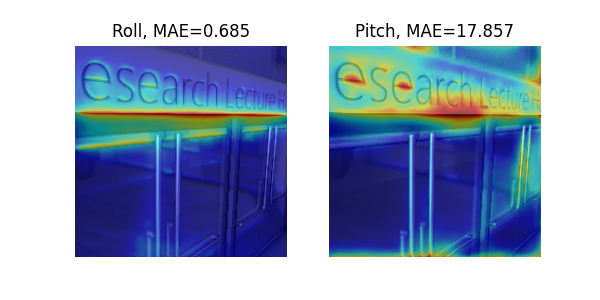
\includegraphics[keepaspectratio, scale=0.55]{./figure/appendix/unknown_env/image_4.png}
    \subcaption{Image Obtained from Office Entrance in Unknown Environment}
  \end{minipage} \\
  \begin{minipage}[htpb]{1.0\linewidth}
    \centering
    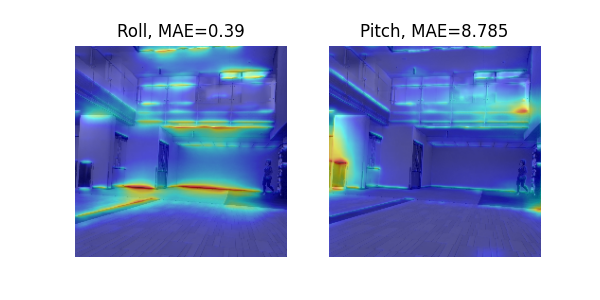
\includegraphics[keepaspectratio, scale=0.55]{./figure/appendix/unknown_env/image_148.png}
    \subcaption{Image Obtained from Corridor in Unknown Environment}\label{fig:roll_example}
  \end{minipage}
  \caption{Images Obtained Using Grad-CAM in Kawai's Method\cite{9708864}}\label{fig:grad_cam}
\end{figure}

\begin{comment}
\begin{figure}[htpb]
\centering
  \begin{minipage}[htpb]{1.0\hsize}
    \centering
    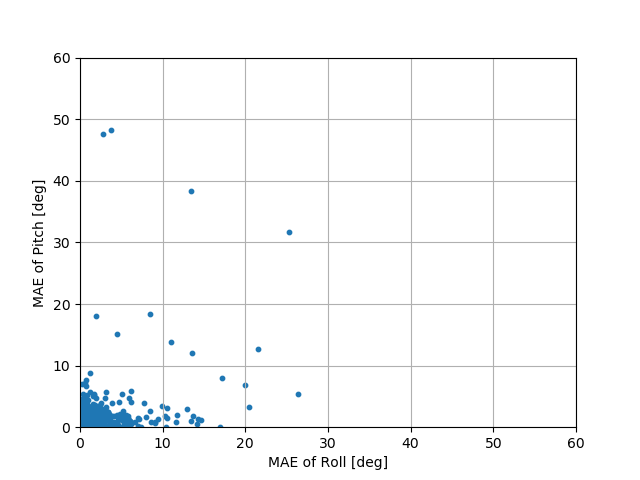
\includegraphics[keepaspectratio, scale=0.38]{./figure/appendix/scatter/MAE_graph_resnet50.png}
    \subcaption{ResNet50}
  \end{minipage} \\
  \begin{minipage}[htpb]{1.0\linewidth}
    \centering
    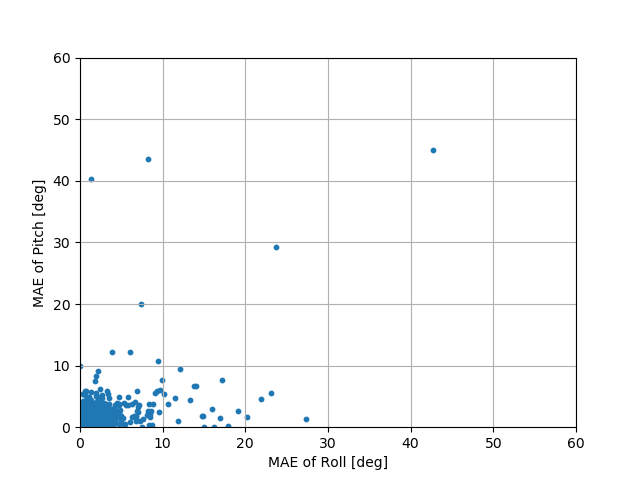
\includegraphics[keepaspectratio, scale=0.38]{./figure/appendix/scatter/MAE_graph_independent_resnet50.png}
    \subcaption{ResNet50(W/O SA-Gate)}
  \end{minipage} \\
  \begin{minipage}[htpb]{1.0\linewidth}
    \centering
    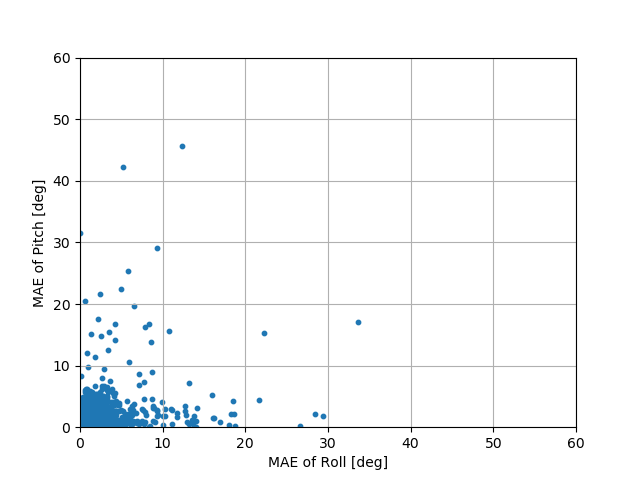
\includegraphics[keepaspectratio, scale=0.38]{./figure/appendix/scatter/MAE_graph_SII2022.png}
    \subcaption{Kawai's Method}
  \end{minipage} \\
  \begin{minipage}[htpb]{1.0\linewidth}
    \centering
    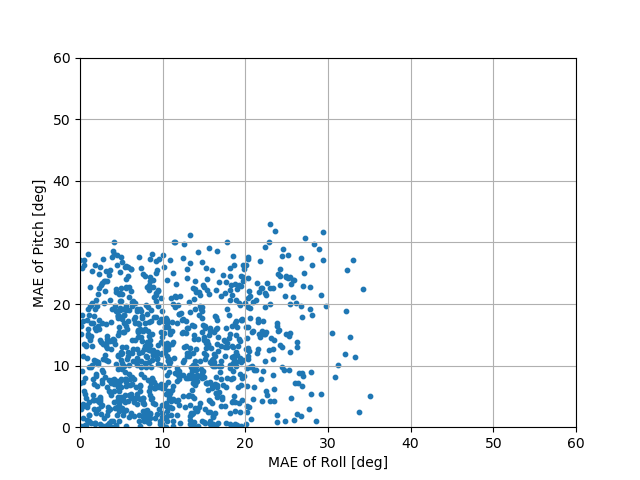
\includegraphics[keepaspectratio, scale=0.38]{./figure/appendix/scatter/MAE_graph_ozaki_mle.png}
    \subcaption{Ozaki's Method(MLE)}
  \end{minipage}
  \caption{MAE of Attitude Estimation in Known Environment}\label{fig:MAE_scatter}
\end{figure}

\begin{figure}[htpb]
\centering
  \begin{minipage}[htpb]{1.0\hsize}
    \centering
    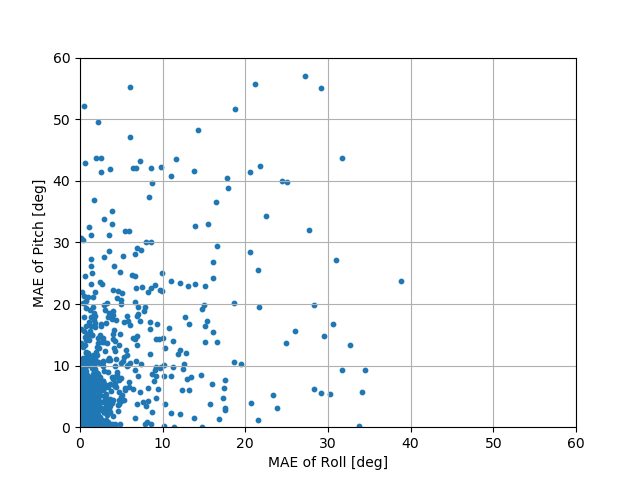
\includegraphics[keepaspectratio, scale=0.38]{./figure/appendix/scatter/MAE_graph_resnet50_unknown.png}
    \subcaption{ResNet50}
  \end{minipage} \\
  \begin{minipage}[htpb]{1.0\linewidth}
    \centering
    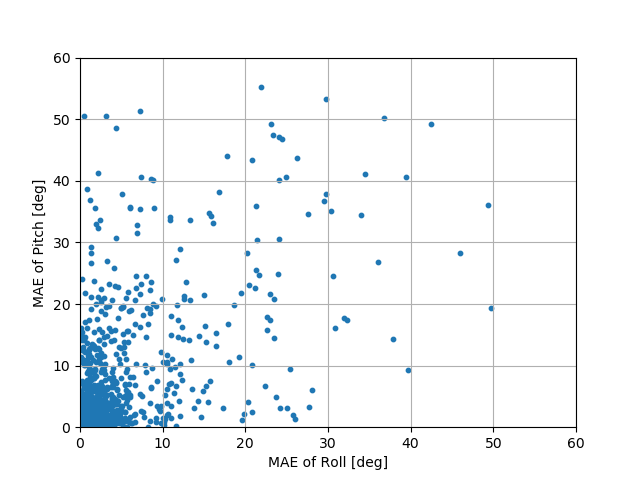
\includegraphics[keepaspectratio, scale=0.38]{./figure/appendix/scatter/MAE_graph_independent_resnet50_unknown.png}
    \subcaption{ResNet50(W/O SA-Gate)}
  \end{minipage} \\
  \begin{minipage}[htpb]{1.0\linewidth}
    \centering
    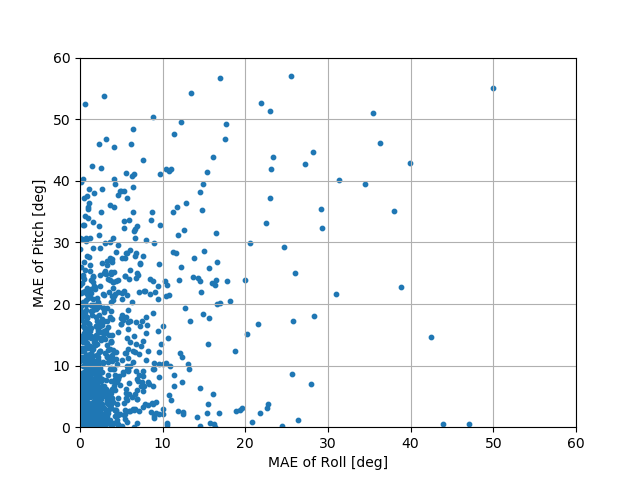
\includegraphics[keepaspectratio, scale=0.38]{./figure/appendix/scatter/MAE_graph_SII2022_unknown.png}
    \subcaption{Kawai's Method}
  \end{minipage} \\
  \begin{minipage}[htpb]{1.0\linewidth}
    \centering
    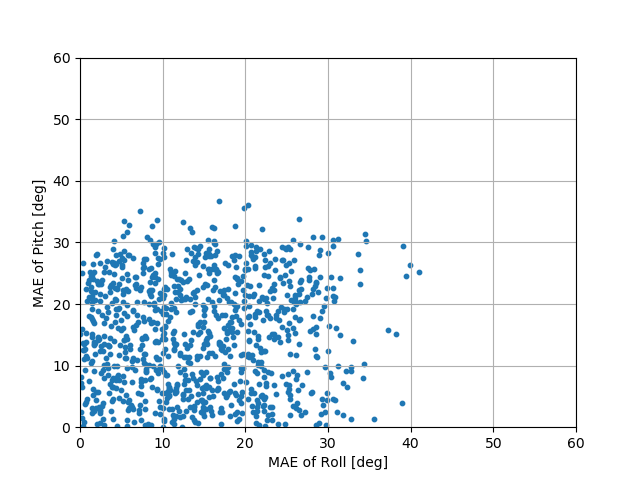
\includegraphics[keepaspectratio, scale=0.38]{./figure/appendix/scatter/MAE_graph_ozaki_mle_unknown.png}
    \subcaption{Ozaki's Method(MLE)}
  \end{minipage}
  \caption{MAE of Attitude Estimation in Unknown Environment}\label{fig:MAE_scatter_unknown}
\end{figure}
\end{comment}


\end{document}
